%%%%%%%%%%%%%%%%%%%%%%%%%%%%%%%%%%%%%%%%%%%%%%%%%%%%%%%%%%%%%%%%%%%%%%%%%%%%%%%%
%2345678901234567890123456789012345678901234567890123456789012345678901234567890
%        1         2         3         4         5         6         7         8

\documentclass[letterpaper, 10 pt, conference]{ieeeconf}  % Comment this line out if you need a4paper

%\documentclass[a4paper, 10pt, conference]{ieeeconf}      % Use this line for a4 paper

\IEEEoverridecommandlockouts                              % This command is only needed if 
% you want to use the \thanks command

\overrideIEEEmargins                                      % Needed to meet printer requirements.

%In case you encounter the following error:
%Error 1010 The PDF file may be corrupt (unable to open PDF file) OR
%Error 1000 An error occurred while parsing a contents stream. Unable to analyze the PDF file.
%This is a known problem with pdfLaTeX conversion filter. The file cannot be opened with acrobat reader
%Please use one of the alternatives below to circumvent this error by uncommenting one or the other
%\pdfobjcompresslevel=0
%\pdfminorversion=4

% See the \addtolength command later in the file to balance the column lengths
% on the last page of the document

% The following packages can be found on http:\\www.ctan.org
%\usepackage{graphics} % for pdf, bitmapped graphics files
%\usepackage{epsfig} % for postscript graphics files
%\usepackage{mathptmx} % assumes new font selection scheme installed
%\usepackage{times} % assumes new font selection scheme installed
%\usepackage{amsmath} % assumes amsmath package installed
%\usepackage{amssymb}  % assumes amsmath package installed

%\usepackage{xcolor}
%\usepackage[switch]{lineno}
\usepackage{amsmath,amsfonts}
\let\labelindent\relax
\usepackage{enumitem}
\usepackage{algorithmic}
\usepackage{algorithm}
\usepackage{array}
\usepackage[caption=false,font=normalsize,labelfont=sf,textfont=sf]{subfig}
\usepackage{textcomp}
\usepackage{stfloats}
\usepackage{verbatim}
\usepackage{graphicx}
\usepackage[noadjust]{cite}
\usepackage[breaklinks]{hyperref}
\usepackage{xurl}
\usepackage{breakurl}
%\usepackage[normalem]{ulem}
%\usepackage[para]{footmisc}
%\usepackage[colorinlistoftodos]{todonotes} % added temporarily by Shane

\title{\LARGE \bf
	Soft Gripping: Specifying for Trustworthiness
}

%%%%%\author{Dhaminda B. Abeywickrama$^{1}$, Nguyen Hao Le$^{2}$, Greg Chance$^{1}$,  Peter D. Winter$^{3}$, Arianna Manzini$^{4}$, \\Alix J. Partridge$^{2}$, Jonathan Ives$^{4}$, John Downer$^{3}$, Graham Deacon$^{5}$, Jonathan Rossiter$^{2}$, Kerstin Eder$^{1}$, Shane Windsor$^{6}$% <-this % stops a space% Albert Author$^{1}$ and Bernard D. Researcher$^{2}$% <-this % stops a space


\author{Dhaminda B. Abeywickrama$^{*1}$, Nguyen Hao Le$^{1}$, Greg Chance$^{1}$,  Peter D. Winter$^{1}$, Arianna Manzini$^{1}$, Alix J. Partridge$^{1}$, \\Jonathan Ives$^{1}$, John Downer$^{1}$, Graham Deacon$^{2}$, Jonathan Rossiter$^{1}$, Kerstin Eder$^{1}$, Shane Windsor$^{1}$% 
\thanks{$^{1}$D. B. Abeywickrama*, N. H. Le, G. Chance, P. D. Winter, A. Manzini, A. J. Partridge, J. Ives, J. Downer, J. Rossiter,  K. Eder and S. Windsor are with the University of Bristol, UK
	{\tt\small firstname.lastname@bristol.ac.uk}}%
\thanks{$^{2}$G. Deacon is with the Robotics Research Team, Ocado Technology, UK
	{\tt\small graham.deacon@ocado.com}}%	
}

%\author{Dhaminda B. Abeywickrama$^{1}$, Nguyen Hao Le$^{2}$, Greg Chance$^{1}$,  Peter D. Winter$^{3}$, Arianna Manzini$^{4}$, \\Alix J. Partridge$^{2}$, Jonathan Ives$^{4}$, John Downer$^{3}$, Graham Deacon$^{5}$, Jonathan Rossiter$^{2}$, Kerstin Eder$^{1}$, Shane Windsor$^{6}$% <-this % stops a space% Albert Author$^{1}$ and Bernard D. Researcher$^{2}$% <-this % stops a space
%	%{*This work was not supported by any organization}% <-this % stops a space
%\thanks{$^{1}$D. B. Abeywickrama*, G. Chance, and K. Eder are with the Department of Computer Science, University of Bristol} 
%	%{\tt\small firstname.lastname@bristol.ac.uk}}\\%
%\thanks{$^{2}$N. H. Le, A. J. Partridge, and J. Rossiter are with the Department of Engineering Mathematics, University of Bristol} 
%	%{\tt\small firstname.lastname@bristol.ac.uk}}%		
%\thanks{$^{3}$P. Winter and J. Downer are with the School of Sociology, University of Bristol}
%	%{\tt\small firstname.lastname@bristol.ac.uk}}%	
%\thanks{$^{4}$A. Manzini and J. Ives are with the Bristol Medical School (PHS), University of Bristol} 
%	%{\tt\small firstname.lastname@bristol.ac.uk}}%				
%\thanks{$^{5}$G. Deacon is with the Robotics Research Team, Ocado Technology, UK} 
%	%{\tt\small firstname.lastname@ocado.com}}%			
%\thanks{$^{6}$S. Windsor is with the Department of Aerospace Engineering, University of Bristol}
%	%{\tt\small firstname.lastname@bristol.ac.uk}}%		
%}

%\author{Albert Author$^{1}$ and Bernard D. Researcher$^{2}$% <-this % stops a space
%	\thanks{*This work was not supported by any organization}% <-this % stops a space
%	\thanks{$^{1}$Albert Author is with Faculty of Electrical Engineering, Mathematics and Computer Science,
%		University of Twente, 7500 AE Enschede, The Netherlands
%		{\tt\small albert.author@papercept.net}}%
%	\thanks{$^{2}$Bernard D. Researcheris with the Department of Electrical Engineering, Wright State University,
%		Dayton, OH 45435, USA
%		{\tt\small b.d.researcher@ieee.org}}%
%}

\begin{document}
	
	
	
	\maketitle
	\thispagestyle{empty}
	\pagestyle{empty}
	
	
	%%%%%%%%%%%%%%%%%%%%%%%%%%%%%%%%%%%%%%%%%%%%%%%%%%%%%%%%%%%%%%%%%%%%%%%%%%%%%%%%
	\begin{abstract}
	Soft robotics is an emerging technology in which engineers create flexible devices for use in a variety of applications.
	In order to advance the wide adoption of soft robots, ensuring their trustworthiness is essential; if soft robots are not trusted, they will not be used to their full potential. 
%	In order to demonstrate trustworthiness, we first need to formulate a \emph{specification} to define what is trustworthy. 
	In order to demonstrate trustworthiness, a \emph{specification} needs to be formulated to define what is trustworthy. 
	However, even for soft robotic grippers, which is one of the most mature areas in soft robotics, the soft robotics community has so far given very little attention to formulating specifications. 
	In this work, we discuss the importance of developing specifications during development of soft robotic systems, and present an extensive example specification for a soft gripper for pick-and-place tasks for grocery items. The proposed specification covers both functional and non-functional requirements, such as reliability, safety, adaptability, predictability, ethics, and regulations.  
	We also highlight the need to promote \emph{verifiability} as a first-class objective in the design of a soft gripper.	
%	Soft robotics is an emerging technology in which engineers create flexible devices for use in a variety of applications.
%	In order to advance the wide adoption of soft robots, ensuring their trustworthiness is essential; if soft robots are not trusted, they will not be used to their full potential. 
%	In order to demonstrate trustworthiness, we first need to formulate a \emph{specification} to define what is trustworthy. However, this has received very little attention from the soft robotics community. 
%	In this work, we discuss the importance of developing specifications during development of soft robotic systems, and present an extensive example specification for a soft gripper for pick-and-place tasks for grocery items. The proposed specification covers both functional and non-functional requirements, such as reliability, safety, adaptability, predictability, ethics, and regulations.  
%	We also highlight the need to promote \emph{verifiability} as a first-class objective in the design of a soft gripper.		
	\end{abstract}
	
%	\begin{IEEEkeywords}
%		Specification, trust, soft gripper, verifiability, evolving functionality, autonomous systems, soft robotics.
%	\end{IEEEkeywords}	
	%%%%%%%%%%%%%%%%%%%%%%%%%%%%%%%%%%%%%%%%%%%%%%%%%%%%%%%%%%%%%%%%%%%%%%%%%%%%%%%%
	\section{INTRODUCTION}\label{introduction}
	
	Soft robotics is an emerging technology in which engineers create flexible devices for use in a variety of applications, such as surgery, prosthetics, space exploration, and grocery picking. 
	%Soft gripping is considered to be one of the most mature areas in soft robotics. % We need to mention soft gripping as we are not providing a specification for a whole soft robitcs system!
	In order to advance the wide adoption of soft robots, ensuring their trustworthiness is essential. 
	%According to Mason \cite{Mason1985}, the central issue in robotic manipulation is how to deal with uncertainty. % has been mentioned as the central issue in robotic manipulation \cite{Mason1985}. % Cut by Shane
	\emph{Trust} may vary, as it can be gained and lost over time, and different research disciplines define trust in different ways; in comparison something is \emph{trustworthy} when it is deserving of trust.

	Autonomous systems (AS) (e.g. soft robotic systems) are considered \emph{trustworthy} when the design, engineering, and operation of these systems generate positive outcomes and mitigate outcomes which can be harmful~\cite{Naiseh2022}.
	% Consider cutting this paragraph - Shane
	Trustworthiness can be dependent on many factors such as: (i) explainability, accountability, and understandability to different users; (ii) robustness in dynamic and uncertain environments; (iii) assurance of their design and operation through verification and validation (V\&V) activities; (iv) confidence in their ability to adapt their functionality; (v) security against attacks; (vi) governance and regulation of their design and operation; and (vii) consideration of ethics and human values in their deployment and use~\cite{Naiseh2022}. 
	
	%The central issue in robotic maltipulation is how to dealwith unccrtainty in Lhe locations and shapes of objects.Humans are cnpablc of effective manipulation in unstructurcd,unprcdictable environments, but robots are not.This deficiency of robots has been addressed in two ways.Most industrial robots finesse the uncertainty problem byorganizing the cnvironme~~t, using special tools to feedand hold parts precisely. A few incluslrial robots usesensors to reduce uncertainty. Most rcsearch laboratoryrobots use the same two approaches-the environment iscon?rolled or scnsors are used.
	
	There are various techniques for demonstrating the trustworthiness of a system, such as formal verification at design-time, monitoring and runtime verification, synthesis, and test-based methods \cite{Abeywickrama2022}. 
	However, common to all these techniques is the need to formulate \emph{specifications}. According to the ISO standard for systems and software engineering vocabulary~\cite{ISO24765:2017}, a \emph{specification} is a detailed formulation that provides ``a definitive description of a system for the purpose of developing or validating the system''. 
	
	\emph{Soft robotic grippers} for manipulating objects are considered to be one of the most mature areas in soft robotics. 
	However, even for this relatively well advanced application area the soft robotics community has so far given very little attention to formulating specifications (e.g. \cite{Shi2023,Cheng2021,Liu2021,Chen2018,Cai2021,Hwang2020,Shin2021}).  Creating a specification as part of a development process is an important step in which the requirements for the system are agreed and defined precisely. % Dhaminda - remvoed formal word as we are not proposing a "formal" specification. It is a high-level, wide-ranging specification.
	The specification then provides a benchmark against which to assess different design options. A well-defined specification also provides a set of criteria against which to verify the performance of the system during design and in operation.
	
	%In addition to formulating a well-defined specification, \emph{verifiability} can be explored to improve the trustworthiness of a soft robotic gripper. 
	In addition to formulating a well-defined specification, a key technique which can explored to improve the trustworthiness of a soft robotic gripper is \emph{verifiability}. % can be explored to improve the trustworthiness of a soft robotic gripper. 
	Verifiability considers verification as an integral part of the system specification and the system design \cite{Mousavi2022}, where it can be promoted to a primary system design objective \cite{Eder2021}. 
	Verifiability will essentially lead to systems that, by their construction, are worthy of our trust. 
	Therefore, the main contributions of this paper are as follows:
	\begin{itemize}
		\item We provide an extensive example specification to ensure the trustworthiness of a soft robotic gripper \cite{Partridge2022} with both functional and non-functional requirements, such as reliability, safety, adaptability, predictability, ethics, and regulations.
		\item We highlight the importance of promoting \emph{verifiability} as a first-class objective in the design of a soft robotic gripper. Also, we provide illustrations of how to formulate verifiable requirements for soft grippers.
		%Also, we provide high-level design guidelines on formulating verifiable requirements. 
	\end{itemize}
	We explore this novel topic using a case study of pick-and-place tasks of grocery items \cite{Triantafyllou2019, Sotiropoulos2018} involving a recycled soft gripper \cite{Partridge2022}. 
	
	The rest of the paper is organised as follows. 
	%In Section~\ref{background-relatedwork}, we provide background and related work, and a brief description of the case study. %to our study. 
	In Section~\ref{background-relatedwork}, we provide background information to this work, key related works, and a brief description of the case study. %to our study. 
	Section~\ref{specification-gripper} provides a detailed specification of a soft gripper, and in Section~\ref{verifiability}, we highlight the significance of promoting verifiability.
	Finally, Section~\ref{summary-conclusions} concludes the paper. 	
	
	\section{BACKGROUND}\label{background-relatedwork}
	
	\subsection{Background}\label{background}
	\subsubsection{Recycled Soft Gripper}
	%[Short Summary of recycled soft gripper paper by \cite{Partridge2022}, which is used in the current study]
	%\textbf{[Alix Partridge to provide this short subsection -- about 300 words]}
	%\\\\\\
	The soft robotic gripper used in this work is a two-finger fluidic elastomer actuator, measuring 12 x 134 x 6 mm \cite{Partridge2022} (see Fig.\ref{gripper}). The gripper is fabricated using a two-part moulding process with a fabric-constraining layer and comprises a mix of 70\% pristine EcoFlex 00-30 silicone elastomer and 30\% recycled EcoFlex 00-30 granules that are 1 mm to 2 mm in size.%, as detailed in \cite{Partridge2022}. %within Partridge et al. (https://ieeexplore.ieee.org/document/9762170).
	
	%\todo[size=\tiny]{Shane: It would be great to add a figure of the gripper here}
	\begin{figure}
		\centering
		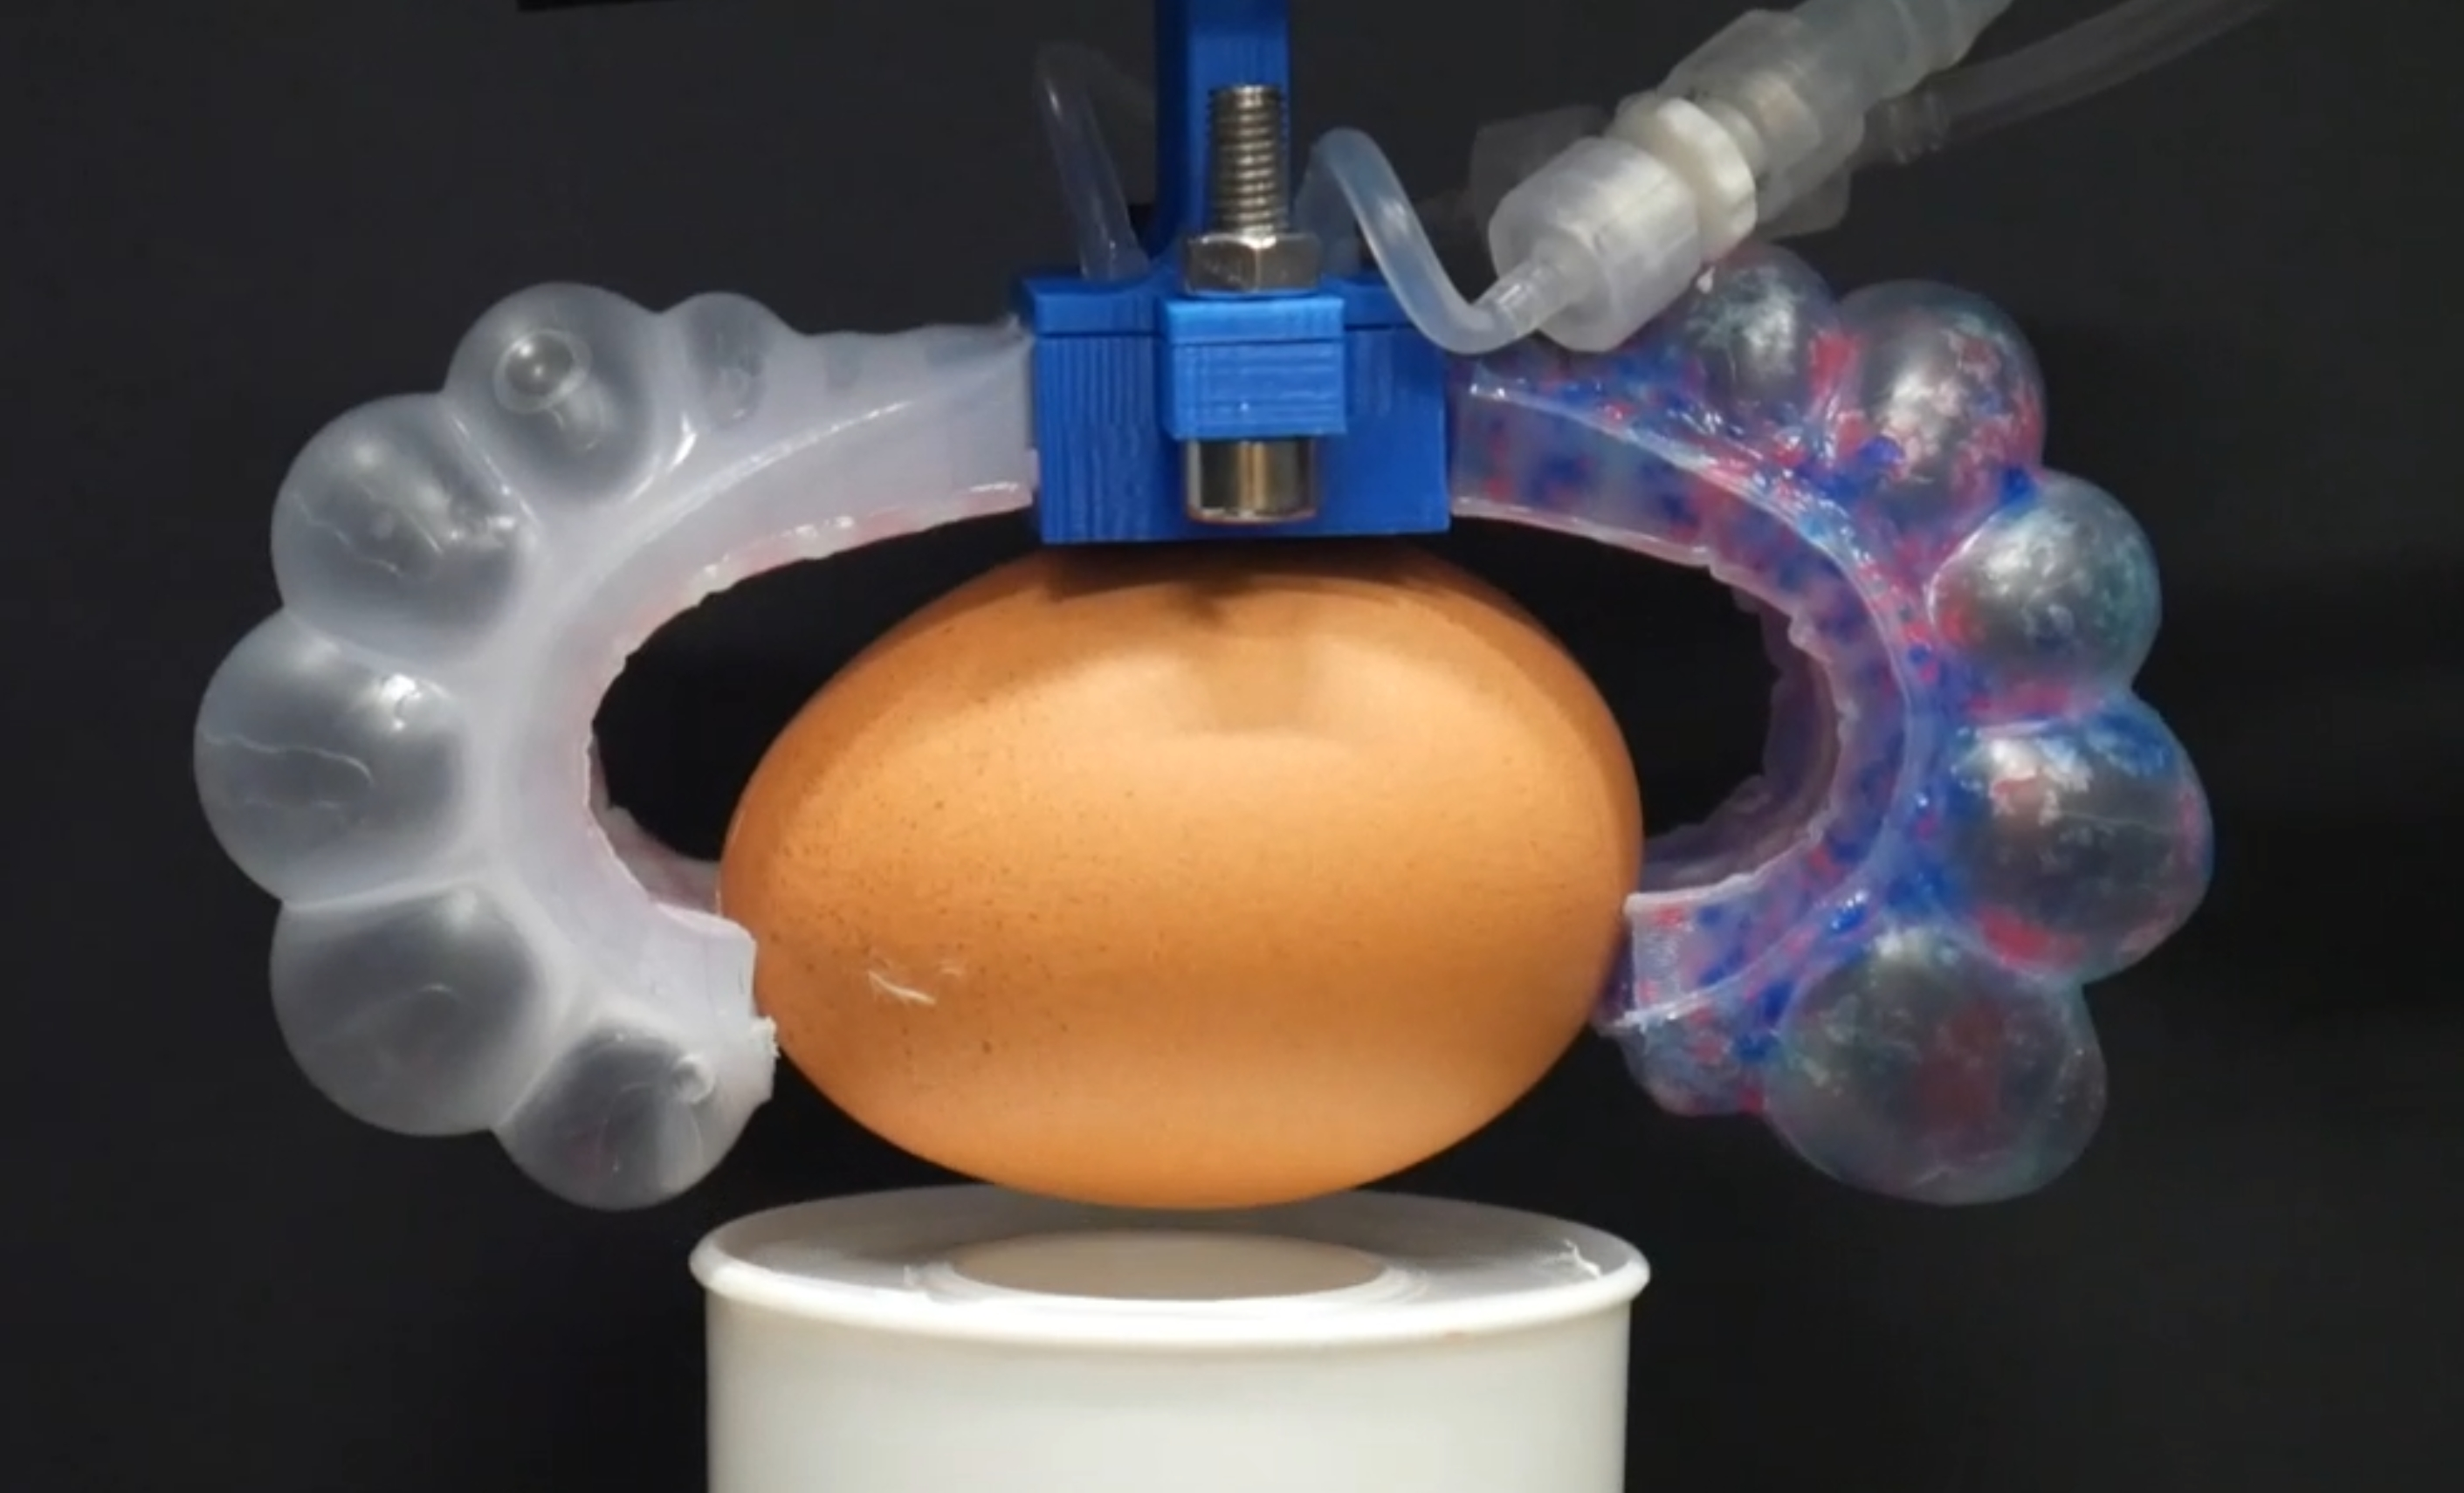
\includegraphics[width=0.4\textwidth]{figures/recycledsoftgripper.jpg}%s[width=0.85\textwidth]
		\caption{A soft gripping system with one pristine silicone finger and a second finger containing 30\% recycle silicone material grasping a fresh egg~\cite{Partridge2022}.}
		\label{gripper}
		%\vspace{-1.3ex}
	\end{figure}
	%	\caption{An interchangeable gripping system shown with one pristine silicone finger and one comprised of 30\% recycle silicone materialSoft gripper. The gripper is shown successfully grasping a fresh egg.}
	
	The operating procedure for the gripper is simple. To actuate the gripper, a positive pressure is introduced to the system that acts to inflate chambers within the gripper body. As the chambers expand, the constraining layer on the base of the gripper prevents expansion of the base of each chamber, while the top of each chamber is free to expand. This differential expansion of top and bottom results in a curving of each chamber, which then leads to an overall curling of the gripper fingers to grasp an object. When vented, this pressure is removed, and the gripper fingers return to a flattened state. 
	
	\subsubsection{Standards} % Condensed by Shane
	Although no direct industry standards have been defined for soft grippers so far, there are several standards in the area of rigid robotics that provide: (i) a set of terminology and definitions for robotic grippers (ISO 14539:2000) and hands \cite{Falco2018}); and (ii) guidance related to the safe spaces, speeds, and forces that a gripping system needs to function (ISO 10218-1/10218-2, and ISO/TS 15066). %In 2022, the ASTM International's committee on robotics, automation, and autonomous systems (F45) formed a new subcommittee on grasping and manipulation, which will develop standards that evaluate performance of grasping type end-effectors.  
	
	\subsection{Related Work}\label{relatedwork}
	Most existing approaches (e.g. \cite{Netzev2023,Hong2022,Bhattacharya2019,Tadakuma2020,Loh2014,Nishikawa2019,Mohan2020}) only describe some technical requirements and parameters of the end-effector to drive its physical design, such as its dimensions, weight, and material properties. For example, Netzev et al.~\cite{Netzev2023} list several technical requirements needed to achieve the desired outcome of their grasping method, such as dimensions and heights of the largest and smallest objects which can be gripped, maximum object weight, and gripping force. 
	Also, most specifications provided for soft grippers only describe their functional requirements (e.g. \cite{Shi2023}), and only a few approaches describe non-functional requirements, such as \emph{adaptability} and \emph{performance} (e.g. \cite{Cheng2021,Liu2021,Chen2018,Cai2021,Hwang2020,Shin2021}).  
	For example, Shi el al. \cite{Shi2023} summarise functional requirements for the characterisation of soft robots with regard to
	their force, dynamics, and stiffness identification. 
	Cheng et al~\cite{Cheng2021} conduct a series of static and dynamic gripping tests that use different forces and fingertip displacements, and demonstrate enhancements to \emph{adaptability} and \emph{performance} of their three-finger soft-rigid gripper. % proposed for low-damage gripping of fragile and soft objects. 
	%In \cite{Shin2021}, the authors propose a soft gripper for smart manufacturing that improves on the Fin Ray finger with enhanced gripping capability. The \emph{performance}, as in gripping weight, of the modified finger has been improved by 40\%.
	However, these works do not cover a wide range of properties which affect the trustworthiness of a soft gripper, as proposed in this work.  
	
	%This section highlights the requirements for the characterisation
	%of soft robotic systems, e.g., with regards to the
	%kinematics/dynamics, stiffness and force capability. These
	%considerations then guide the platform design.
	%we summarised the functionality requirements
	%for the characterisation of soft robots with regard to
	%their kinematics/dynamics, force and stiffness identification.
	
	%lists several technical requirements which are crucial
	%to achieve the desired outcome of blind grasping. Notably,
	%requirements such as the gripping force, payload and object
	%dimensions, are due to the limitations of the robot and its
	%gripper actuation mechanism.
	
	%Most existing works (e.g. \cite{Cheng2021,Liu2021,Chen2018,Cai2021,Hwang2020,Shin2021}) describe improving a trustworthiness property like \emph{adaptability} or \emph{performance} of a soft gripper. Furthermore, most specifications proposed for soft robotics grippers (e.g. \cite{Hong2022,Bhattacharya2019,Tadakuma2020,Loh2014,Nishikawa2019,Mohan2020}) only describe some parameters of the end-effector, such as their dimensions, weight, and material properties.
	%These works do not cover a broad range of properties for trustworthiness, as considered in our study.  
	%For example, \cite{Cheng2021} conduct a series of static and dynamic gripping tests that use different forces and fingertip displacements, and demonstrate enhancements to \emph{performance} and \emph{adaptability} of their three-finger soft-rigid gripper proposed for low-damage gripping of fragile and soft objects. 
	%In \cite{Shin2021}, the authors propose a soft gripper for smart manufacturing that improves on the Fin Ray finger with enhanced gripping capability. The \emph{performance}, as in gripping weight, of the modified finger has been improved by 40\%. 
	
	%A key limitation of the existing approaches is that they only cover a very limited range of properties, such as performance and adaptability.  
	%Furthermore, most existing works describe only some parameters of the end-effector, such as its dimensions, weight, and material. 
	
	%As discussed, most existing works (e.g. \cite{Cheng2021,Liu2021,Chen2018,Cai2021,Hwang2020,Shin2021}) describe improving \emph{adaptability} or \emph{performance} of a soft gripper. However, these works do not cover a broad range of properties for trustworthiness, as considered in our study. %one or two trustworthiness properties of a soft gripper like 
	%Furthermore, most existing approaches (e.g. \cite{Hong2022,Bhattacharya2019,Tadakuma2020,Loh2014,Nishikawa2019,Mohan2020}) only describe some parameters of the end-effector, such as their dimensions, weight, and material properties.
	%
	
	%Besides functional requirements of the fingers, the technical
	%requirements drive its physical design. In particular,
	%Table I lists several technical requirements which are crucial
	%to achieve the desired outcome of blind grasping. Notably,
	%requirements such as the gripping force, payload and object
	%dimensions, are due to the limitations of the robot and its
	%gripper actuation mechanism.
	
	
	%\todo[size=\tiny]{Shane: This needs to be summarized rather than be a description of seperate papers. Needs to be condensed to make room for figure and additional subsection on why we need specification.}
	%
	%In \cite{Cheng2021}, the authors propose a three-finger soft-rigid gripper actuated by a soft pneumatic actuator for the low-damage gripping of fragile and soft objects. 
	%By conducting a series of static and dynamic gripping tests that use different forces and fingertip displacements, the authors demonstrate enhancements to the \emph{performance} and \emph{adaptability} of their gripper.  %linear-extension 
	%
	%A compliant soft robotic gripper for grasping and manipulating objects is proposed in \cite{Liu2021}.  This underactuated gripper is able to undertake practical in-hand manipulation of caps despite significiant uncertainty in object orientation and finger position.   
	%The core issue being addressed is \emph{adaptability} that achieves tolerance and dexterity for manipulating objects of various sizes, shapes, masses, and positions/orientations. 
	%The grasping tests conducted demonstrate that the soft finger can conform to the object?s surface with stable grasping and environmental endurance. 
	%
	%In\cite{Chen2018}, the authors synthesise a soft cable-driven gripper by recasting its mechanical design as a topology optimisation problem. 
	%They perform several fatigue, blocking force, and grasping tests to evaluate the \emph{performance} of their gripper.  
	%The results of the grasping tests reveal that their optimised gripper can handle a wide range of unknown objects of different shapes and weights with different grasping modes (i.e. power grips, precision grips, and a combination of both).
	%
	%In another related work \cite{Cai2021}, a pneumatic webbed soft gripper has been developed and evaluated to grasp unstructured and fragile objects. 
	%The authors present experimental results of grasping delicate objects (e.g. egg, strawberry, candy, and knife) to demonstrate the \emph{safety} and \emph{adaptability} of their webbed soft gripper. %%%%%%% for fragile and crisp objects.
	%
	%A reinforced soft gripper is proposed in \cite{Hwang2020} with a mechanically strengthened electro-adhesion pad and a multi-layered dielectric elastomer actuator. This soft gripper has two fingers and it can grasp various shapes of objects, such as hexahedral, spherical, cylindrical, and flat structures, thus demonstrating \emph{adaptability}. Also, the gripper with a mass of 6.2 g, could hold and move objects weighing 625 g. 
	%
	%In \cite{Shin2021}, the authors propose a soft gripper for smart manufacturing that improves on the Fin Ray finger with enhanced gripping capability. The \emph{performance}, as in gripping weight, of the modified finger has been improved by 40\%. The authors perform gripping tests for 17 rigid and soft objects.
	%
	%As discussed, most existing works (e.g. \cite{Cheng2021,Liu2021,Chen2018,Cai2021,Hwang2020,Shin2021}) describe improving \emph{adaptability} or \emph{performance} of a soft gripper. However, these works do not cover a broad range of properties for trustworthiness, as considered in our study. %%%one or two trustworthiness properties of a soft gripper like 
	%Furthermore, most existing approaches (e.g. \cite{Hong2022,Bhattacharya2019,Tadakuma2020,Loh2014,Nishikawa2019,Mohan2020}) only describe some parameters of the end-effector, such as their dimensions, weight, and material properties.%%%%%, and no work proposes a wide-ranging specification for trustworthiness.%, as proposed in our study.
	
	\subsection{Case Study: Pick-and-Place Tasks of Grocery Items}
	Let us consider an automated warehouse, where items are picked from storage crates using a soft robotic gripper and are then placed in delivery crates for delivery. 
	An example grocery use case is that of Ocado, which is considered the world's largest online-only supermarket \cite{Triantafyllou2019, Sotiropoulos2018}. 
	A range of uncertainties make automation of this process challenging: (i) items can vary in their shape, size, packaging, and orientation; (ii) some items are fragile or deformable; (iii) geometrically constrained and relatively cluttered operating environment~\cite{Triantafyllou2019}; (iv) manufacturing inconsistencies (low tolerances) in the gripper; and (v) elastic nature of the materials used in the gripper, which can lead to performance degradation.
	
	In this case study, we consider four \emph{classes} of items: (i) \emph{soft-fragile} items (e.g. cake, bread, strawberry, bayberry), (ii) \emph{soft-non-fragile} items (e.g. dish sponge), (iii) \emph{hard-fragile} items (e.g. light bulb, egg), (iv) \emph{hard-non-fragile} items (e.g. plastic spoon). 
	The objects being picked can be regular-shaped items (e.g. sphere, cube, cone, pyramid, cylinder) or irregular-shaped ones (e.g. strawberries). The robotic pick-and-place task can be structured into a pipeline of four main tasks: (i) pre-grasping, (ii) ascension (grasping), (iii) translation (transport), and (iv) descension (placement). 

\section{SPECIFICATION OF A SOFT GRIPPER}\label{specification-gripper}
	In this section, we present an example of a wide-ranging specification with functional and non-functional properties which affect the trustworthiness of a soft gripper. We define these in terms of predictability, reliability, adaptability, safety, ethics, and regulations (see Fig.\ref{SR-spec}). 
	
	This example specification was developed through consultation with requirements engineers, soft robotic developers, industrial users, ethicists, and sociologists. It is an example of the aspects that may need to be specified for a soft gripper rather than an exhaustive specification for every aspect of the system. 
	The specification includes functional requirements -- those that specify behaviour the system shall perform~\cite{ISO24765:2017}; and non-functional requirements -- those that specify not what the system will do but how it will do it (quality attributes)~\cite{ISO24765:2017}.
	%The specification includes functional requirements -- those needed to achieve the technical task, and non-functional requirements -- those related to the broader operation of the system, such as ethical and regulatory considerations. 
	% added by Shane  ; edited by Dhaminda
	%This example specification was developed through consultation with soft robotic developers, industrial users, ethicists, sociologists and from published requirements. Dhaminda - I have edited this sentece. I don't think we took "any published requirements". All the shall statements in the paper we developed. 
	The engineering requirements (iii a--d) are formulated as `shall' statements following the guidance on writing good requirements \cite{NASA2007}, and the ethics and the regulatory requirements (iii e--f) are discussed using key frameworks from ethics~\cite{Porter2023} and social science~\cite{Macrae2022}. 
	
	Below we define the set of requirements \{RQx\} for a soft gripper across these six properties.
	We define the boundaries to measure the success of gripping an item using the conventional bounds of 95\% for success and 5\% for failure. 
	Also, in the following, whenever a performance threshold is given, where possible we aim to provide a reference from a published work/experiment. 
	\begin{figure*}
		\centering
		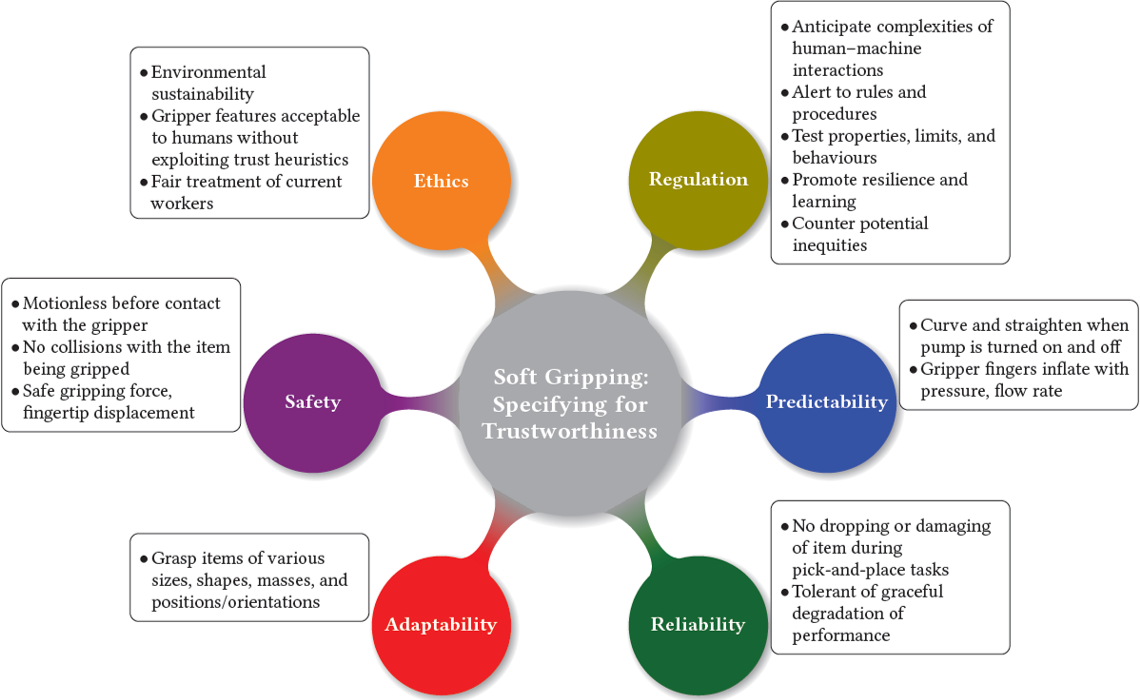
\includegraphics[width=0.75\textwidth]{figures/properties}%soft-t-v2.png
		\caption{Soft gripper: Specifying for trustworthiness. Core properties (coloured) are evaluated through a range of practical evaluations (boxes). }
		\label{SR-spec}
	\end{figure*}
	
	\paragraph{\textbf{Predictability}}\label{predictability}
	Predictability is ``a property of interaction concerning the degree of confidence with which a user can determine the effect subsequent task execution will have on the achievement of the goal"~\cite{Abowd1991}. A soft gripper needs to be predictable in its behaviour, so it can build a degree of confidence and trust for the end-user.  
	\begin{itemize}[leftmargin=*]
		\item RQ1.1: The fingers of the gripper \emph{shall} curve when inflated (pump turned on).  
		\item RQ1.2: The fingers of the gripper \emph{shall} straighten when deflated (pump turned off).  
		\item RQ1.3: The curvature of a finger \emph{shall} be proportional to its internal pressure. 
		\item RQ1.4: The gripper \emph{shall} grasp, transport, and place an item successfully with a repeatability of $\ge$95\%.
		%	\item RQ1.4: The gripper \emph{shall} grasp, transport and place an item under same conditions with a $\ge$95\% pick-and-place repeatability.
		%	\item RQ1.4: The fingers \emph{shall} be in a stable state -- pre-pressurized/inflated 10 times, prior to being used.  
		\item RQ1.5: The fingers \emph{shall} be inflated with a pressure between 3 and 4 psi pressure range \cite{Partridge2022}. 
		\item RQ1.6: The fingers \emph{shall} be inflated with a flow rate between 2 and 3.2 L/min range \cite{DEWIN2022}.
	\end{itemize}
	
	\paragraph{\textbf{Reliability}}\label{reliability}
	\emph{Reliability} is defined as the ``ability of a system or component to perform its required functions under stated conditions for a specified period of time" \cite{ISO24765:2017}. A soft gripper needs to be reliable by not dropping or damaging items during pick-and-place tasks, and should be tolerant of graceful degradation of performance.
	
	\begin{itemize}[leftmargin=*]
		\item RQ2.1: The gripper \emph{shall} hold the item being gripped without damaging it. 
		\item RQ2.2: The gripper \emph{shall} hold the item being gripped without dropping it for at least 10 seconds 95\% of the time (\cite{Sotiropoulos2018}, p. 652).
		\item RQ2.3: The gripper \emph{shall} successfully maintain grasp during the translation of the gripped item for a maximum velocity and acceleration of 0.03 m/s and 0.15 m/s$^2$ (\cite{Triantafyllou2019}; \cite{Cheng2021}).
		\item RQ2.4: The gripper \emph{shall} successfully grasp when the rate of inflation is in the range of 2-3.2 L/min \cite{DEWIN2022}.
		\item RQ2.5: The gripper \emph{shall} experience $\le$ 5\% increase in the dropping of an item across 100 hours of operation (graceful degradation). %(comment by SW: consider degradation rate instead?) 
		\item RQ2.6: The gripper \emph{shall} experience $\le$ 5\% increase in the damaging of an item across 100 hours of operation (graceful degradation).  %(comment by SW: consider degradation rate instead?) 
	\end{itemize}
	\paragraph{\textbf{Adaptability}} \label{adaptability}
	\emph{Adaptability} is defined as the ``degree to which a product or system can effectively and efficiently be adapted for different or evolving hardware, software or other operational or usage environments" \cite{ISO24765:2017}. In a soft gripper, \emph{adaptability} is key to manipulating objects of various sizes, shapes, masses, and positions/orientations. 
	\begin{itemize}[leftmargin=*]
		\item RQ3.1: The gripper \emph{shall} hold items of different sizes up to a maximum of 95\% of the opening width of the two fingers without dropping them for at least 10 seconds 95\% of the time.
		\item RQ3.2: The gripper \emph{shall} hold items of different shapes (e.g. sphere, cube, cone, pyramid, cylinder) without dropping them for at least 10 seconds 95\% of the time.
		\item RQ3.3: The gripper \emph{shall} hold items, which can be of regular or irregular shape (e.g. soft-fragile items like strawberry), without dropping them for at least 10 seconds 95\% of the time.
		\item RQ3.4: The gripper \emph{shall} hold an item independent of its orientation without dropping it for at least 10 seconds 95\% of the time. 	  
	\end{itemize}
	
	\paragraph{\textbf{Safety}}\label{safety}
	\emph{Safety} is defined as an ``expectation that a system does not, under defined conditions, lead to a state in which human life, health, property, or the environment is endangered" \cite{ISO24765:2017}. 
	In this work, we consider safety from the perspective of the item being gripped where physical damage should be avoided during pick-and-place tasks. % and not from any physical harm to a human.
	\begin{itemize}[leftmargin=*]
		\item RQ4.1: The item being gripped \emph{shall} be motionless (to minimise harm) before contact with the gripper. 
		\item RQ4.2: The gripping system \emph{shall} not collide with the item being gripped. 
		\item RQ4.3: The gripping system \emph{shall} only make contact with the item using the gripper.
		\item RQ4.4: When grasping a hard-fragile item (e.g. light bulb, egg), the soft actuator \emph{shall} be inflated until the gripping force does not exceed 2 N (\cite{Cheng2021}).
		\item RQ4.5: When grasping a soft-fragile item like cake or bread, the soft actuator \emph{shall} be inflated until the fingertip displacement does not exceed 3 mm (\cite{Cheng2021}).
		\item RQ4.6: When grasping a soft-fragile item like strawberry or raspberry, the soft actuator \emph{shall} be inflated until the gripping force does not exceed 1 N and the fingertip displacement does not exceed 1 mm (\cite{Cheng2021}, p. 14).
	\end{itemize}
	
	\paragraph{\textbf{Ethics}}\label{ethics}
	Human values inform the design and use of technologies, and the resulting distribution of benefits and burdens, and those values underpin system trustworthiness. Rather than \emph{describing} whether people \emph{trust} a technology, ethicists are interested in \emph{prescribing} whether they \emph{should trust} it. Below are some key ethical requirements for specifying for trustworthiness in a soft gripper in pick-and-place tasks.
	\begin{itemize}[leftmargin=*]
		\item RQ5.1: The gripper \emph{shall} 
		be environmentally sustainable. 
		\item RQ5.2: The gripper \emph{shall} avoid distressing human workers.
		\item RQ5.3: The gripper \emph{shall} avoid exploiting humans' trust heuristics.
		\item RQ5.4: The gripper \emph{shall} accommodate fair treatment of current human workers.
	\end{itemize}
	
	The use of a recycled gripper may make its manufacturers or the company deploying it \emph{look like} they care for the environment and so appear more trustworthy, thus increasing public trust in them. However, such a system may not perform as well as, or may degrade more rapidly than, a system made of virgin material, thus making it more likely for items to be dropped or damaged. When the item being gripped is food, the risk of food waste increases, with detrimental implications for the environment. Unless the above reliability requirements are met by design, the use of a recycled gripper could be a form of `greenwashing'~\cite{delmas2011drivers}.    
	
	Moreover, while technical requirements aim to prevent \emph{physical} harm, specifying for trustworthiness should include considerations of potential \emph{psychological} harm \cite{Porter2023}. By replicating a human feature (fingers/hand) and behaviour (gripping) without being human-like enough to convince, a soft gripper risks could produce an uncanny valley effect \cite{moore2012bayesian} that distresses humans. User studies should identify gripper shapes that are acceptable to humans, whilst aiming for optimal gripping.  
	
	Simultaneously, the biomimetic features of soft grippers risk exploiting humans' trust heuristics, which make them trust things they are already familiar with \cite{Manzini}. As the use of soft robotics technologies can result in many unsafe conditions (e.g. material failure, crushing~\cite{abidi2017intrinsic}), trust in the safety of a soft gripper could be misplaced if it was only based on a sense of familiarity with it. To reduce risks of harm, the robot area should be clearly separated from the space accessible to humans.
	
	\paragraph{\textbf{Regulations}}\label{regulation}
	To design successful AS we must formulate specifications from a \emph{sociotechnical} perspective, that is not only regarding the technical features of the system as discussed in III a--d, but also social features of its development and use as fundamentally interrelated. So, in designing a soft gripper for pick-and-place tasks for grocery items, we need to be sensitive to sociotechnical requirements, where the analysis of human, social, cultural, and organisational dynamics can help us think about why and how failures happen with regards to AS. In this context, Macrae's \cite{Macrae2022} `SOTEC' (structural, organisational, technological, epistemic, and cultural) framework is a useful approach for identifying domains of sociotechnical risk in AS. The schema can help inform emergent regulation by identifying often-neglected risks. Below we outline each category and consider its application to the pick-and-place tasks of grocery items.
	%autonomous and intelligent systems
	
	%\emph{Structural} sources of risk arise from interactions between different human and nonhuman elements that amplify or transmit local failures in a system in ways that disable the entire system. 
	\emph{Structural} sources of risk arise from interactions between human and nonhuman elements in a system.
	In a pick-and-place task, such risks may arise from unanticipated disruptions, such as a human moving a grocery item, confusing the perception system. Regulatory requirements should ensure that the system anticipates and accommodates the complexities of human-machine interactions.
	
	\emph{Organisational} sources of risk emerge when organisational structures, such as rules and expectations, are insensitive to the vagaries of real human behaviour. For example, protocols for checking capabilities required for grasping might presuppose an unrealistic degree of diligence. Regulatory requirements should be alert to the practical dimensions of potential rules and procedures.
	
	\emph{Technological} sources of risk arise from the shortcomings of the system itself. These are the myriad risks that engineers would conventionally consider as part of their work. In the context of the pick-and-place pipeline, there may be concern about recycled materials degrading and shedding particles into food. Regulators should ensure that designers effectively test the properties of the recycled materials, their limits and behaviours.
	%Regulators should ensure that designers effectively test properties, limits and behaviors.
	
	\emph{Epistemic} sources of risk arise from the inherent indeterminacies of knowledge, which create pockets of ignorance that hide unexpected hazards. Such pockets are difficult to mitigate (since we don't know what we don't know) but it can be anticipated that the system's attempt to grasp the object could fail for unexpected reasons, and tailor regulatory provisions in ways that promote resilience and learning. 
	
	\emph{Cultural} sources of risk arise from collective values (beliefs and norms) that frame and influence AS design and operation. For instance, if a gripper's grasp is optimised for western food items (e.g. tins), this may mean that it underperforms for eastern food items (e.g. bags), negatively affecting a minority of stakeholders. Regulatory requirements must reflect critically on their underlying values, and work to counter potential inequities. 
	
	\section{VERIFIABILITY OF A SOFT GRIPPER} \label{verifiability}
	%\todo[size=\tiny]{Shane: I think we need a linking sentence or two here to help reader relate specification to verification. Just a high level overview of how the two are related.}
	In addition to formulating a well-defined specification as discussed in the preceding section, \emph{verifiability} can also be explored to improve the trustworthiness of a soft robotic gripper. 
	Verification is the process that can be used to gain confidence in the correctness of a system with respect to its specification~\cite{Bergeron2000}. 
	Verifiability can be achieved by considering verification early, such as during specification and system design \cite{Mousavi2022}, where it can be promoted to a primary system design objective \cite{Eder2021}.
	A unified and holistic approach to verifiability will lead to systems that are, by their construction, are worthy of our trust \cite{Mousavi2022}. 
	
	For a system to be {\em verifiable\/}, a person or a tool needs to be able to check its correctness~\cite{ISO24765:2017} with respect to its requirements and specification \cite{Abeywickrama2022}. 
	The main challenge is in specifying and designing the system in such a way that this process is made as easy and intuitive as possible.
	%
	For AS in particular, specific challenges~\cite{Abeywickrama2022} include: 
	%
	(i) capturing and formalising requirements including functionality, safety, security, performance and, beyond these, any additional non-functional requirements purely needed to demonstrate trustworthiness; 
	%	 
	(ii) handling flexibility, adaptation, and learning; and 
	%
	(iii) managing the inherent complexity and heterogeneity of both the AS and the environment it operates in. 
	
	Gerson~\cite{Gerson1993} identifies several techniques for ensuring verifiability: bounding the verification task, prioritising effort, ensuring traceability, and breaking down high-level requirements into verifiable portions. 
	According to Gerson~\cite{Gerson1993}, formulating requirements for verifiability should go far beyond avoiding negative requirements and including numerical tolerances, but also aim to \emph{design for verifiability}. 
	This is because the ultimate purpose of specifications is verifying that the end product exhibits the intended properties. 
	This requires the intended properties to be \emph{demonstrable}; that is, knowledge of the end result needs to be attainable. 
	In this work, we have considered this early when formulating requirements, by planning and confirming how these properties can be verified subsequently (see Table~\ref{Table:Verifiability}). 
	For example, requirements RQ1.1, 1.2, 1.4, 2.1, 2.2, and 2.4 can be verified by \emph{observing} the gripping system during operation. 
	Observation is ``a technique that provides a direct way of viewing individuals in their environment performing their jobs or tasks and carrying out processes"~\cite{ISO24765:2017}.
	Let us describe a unit test that can be conducted to verify requirement RQ1.5. 
	A two-fingered soft pneumatic gripper can be fabricated as proposed in \cite{Partridge2022} using 30\% recycled material. 
	One can use black pigments to track the chambers and granules, and red pigments to track the curvature of the constraining layer. 
	The fingers can be actuated and their motion can be captured with a camera. 
	The curvature with time can be determined by conducting image processing on the video, and the internal pressure with time can be monitored.
	
	%Following the guidance on writing good requirements provided in \cite{NASA2007}, the requirements in Section~\ref{specification-gripper} have been formulated positively (i.e. use of \emph{shall} statements as opposed to \emph{shall not} statements). 
	As mentioned previously, the engineering requirements (iii a--d) have been formulated by following the guidance provided in~\cite{NASA2007}. 
	On the one hand, most engineering requirements contain numeric tolerances (verifiable). 
	For example, RQ1.5 identifies a specific pressure range. 
	Similarly, in RQ4.4, we identify a maximum value of 2 N for gripping force when gripping a hard-fragile item. 
	On the other hand, there are several high-level requirements which need to be refined into verifiable terms before any verification method can be applied.  
	For instance, requirements RQ1.1--1.3 have been formulated at a high-level because the amount of curvature and straightening of a finger can often be dependent on the application. 
	In order to be verifiable, we can refine RQ1.1 as: the fingers of the gripper \emph{shall} curve within 2\% of a curve of 10 cm radius when inflated. 
	Similarly, we can refine requirement RQ4.2 as: no part of the body of gripping system \emph{shall} have a position equal to the position of the item being grasped. 
	This can be verified by monitoring the distance between each of the joints of the gripping system to ensure that there is no collision between the body of the gripping system and the item. 
	Meanwhile, with respect to RQ4.1, one does not need to impose an initial velocity on the food item in the test bed, so this requirement can be met by design (i.e. no need to formally verify or monitor it). Thus, the above examples illustrate two versions of the specification for a soft robotic gripper -- one a \emph{verifiable} one from the start (e.g. RQ1.5, RQ4.4); and the other a more \emph{high-level}, unrefined one (e.g. RQ1.1, RQ4.2), for which, through examples, we demonstrate how to make it verifiable. In this manner, this work not only provides a wide-ranging specification for a pick-and-place application, but also provides illustrations of how to formulate verifiable requirements for soft grippers. 

%	The above examples show how a specification can be written to be verifiable based on an initial high-level requirement.
%	In this manner, this work not only provides a wide-ranging specification for a pick-and-place application, but also provides illustrations of how to formulate verifiable requirements for soft robotics. 
 
%	As discussed, this work provides two versions of the specification for a soft robotic gripper -- one a \emph{verifiable} one from the start, and the other a more \emph{high-level} one, for which, through examples, we demonstrate how to make it verifiable. 
%	By doing this, we show the difference between a high-level requirement and its verifiable version. 
%	In this manner, this work not only provides a wide-ranging specification for a pick-and-place application, but goes a step further by providing high-level design guidelines on formulating verifiable requirements for the soft robotics community. % requirements verifiable.
	
	\begin{table}%[!t]
		\centering
		\caption{\label{Table:Verifiability} Soft-gripper requirements and verification methods.}
		\begin{tabular}{|p{16mm}|p{65mm}|}
			\hline
			\textbf{Requirements} & \textbf{Verification Method} \\ 
			\hline
			RQ1.1,1.2,1.4, 2.1,2.2,2.4 & \emph{Observation} during operation\\%Visual Inspection \\
			\hline
			RQ1.3,1.5 & \emph{Practical tests}: unit testing  \\
			\hline
			RQ2.3 & \emph{Practical tests}: edge-case testing \\
			\hline
			RQ2.5,2.6 & \emph{Practical tests}: life-cycle testing \\
			\hline
			RQ3.1,3.2,3.3 & \emph{Practical tests}: repeated testing, and \emph{Observation} \\
			\hline
			RQ4.1 & \emph{Measurement}: vision camera, and \emph{Observation}  \\ 
			\hline
			RQ4.2 & \emph{Measurement}: force torque sensor \\ 
			\hline
			RQ4.3 & \emph{Measurement}: force torque sensor and vision camera  \\ 
			\hline
			RQ4.4 & \emph{Practical tests}: functional test\\ 
			\hline
			RQ4.5 & \emph{Measurement}: displacement sensor   \\ 
			\hline
			RQ4.6 & Both \emph{Practical tests}: functional test, and \emph{Measurement}: displacement sensor \\ 
			\hline
		\end{tabular}\vspace{-2.7ex}
	\end{table}

\section{CONCLUSION} \label{summary-conclusions}%Summary and Conclusions
	As soft robotics continue to expand into new and diverse industries it is important to consider the design processes used, particularly the development of detailed specifications which can be used to define the requirements for a system and ensure that both functional and non-functional aspects are considered from an early stage of the development process.
	Within soft robotics, soft gripping is considered to be one of the most mature areas. 
	For wider adoption and acceptability, we must build soft grippers worthy of our trust. 
	In this context, this work proposed an extensive \emph{specification} for a soft gripper covering several functional and non-functional properties, including predictability, reliability, adaptability, safety, ethics, and regulations. 
	In addition, we promoted the notion of \emph{verifiability} of a soft gripper as a first-class design objective, and provided illustrations of how to formulate verifiable requirements.  
	%In addition, we promoted the notion of \emph{verifiability} of a soft gripper as a first-class design objective, and identified several high-level design guidelines on formulating verifiable requirements. 
	This work was explored using the pick-and-place tasks of grocery items in an automated warehouse. 
 We conclude that specifying for trustworthiness in soft robotics as complete systems for real world applications should use a multi-disciplinary approach with inputs from a range of experts including soft roboticists and engineers, as well as experts from the social sciences and humanities.  A multi-disciplinary approach will help ensure that any specification covers both functional and non-functional requirements and will help develop trustworthy soft robots.
 
	%We conclude that specifying for trustworthiness in a soft gripper requires advances in engineering, informed by new insights from social sciences and humanities research. Thus, tackling this specification challenge necessitates a multi-disciplinary approach with close collaboration of soft roboticists, engineers, and computer scientists with experts from psychology, sociology, law, politics, and economics, as well as ethics and philosophy.
	
	\addtolength{\textheight}{-12cm}   % This command serves to balance the column lengths
	% on the last page of the document manually. It shortens
	% the textheight of the last page by a suitable amount.
	% This command does not take effect until the next page
	% so it should come on the page before the last. Make
	% sure that you do not shorten the textheight too much.
	
	%%%%%%%%%%%%%%%%%%%%%%%%%%%%%%%%%%%%%%%%%%%%%%%%%%%%%%%%%%%%%%%%%%%%%%%%%%%%%%%%
	
	\section*{ACKNOWLEDGMENT}
	This work has been supported by the UKRI Trustworthy Autonomous Systems Node in Functionality under Grant EP/V026518/1. J.R.\ is supported by EPSRC grants EP/R02961X/1, EP/S026096/1, EP/V062158/1, and EP/T020792/1, and the Royal Academy of Engineering through the Chair in Emerging Technologies scheme, grant CiET17182$\backslash$22.
	%The work presented in this paper has been supported by the UK Engineering and Physical Sciences Research Council (EPSRC) under the grant [EP/V026518/1]. JR is supported by EPSRC grants EP/R02961X/1, EP/S026096/1, EP/V062158/1, and EP/T020792/1, and the Royal Academy of Engineering through the Chair in Emerging Technologies scheme, grant CiET17182$\backslash$22.
	
	%%%%%%%%%%%%%%%%%%%%%%%%%%%%%%%%%%%%%%%%%%%%%%%%%%%%%%%%%%%%%%%%%%%%%%%%%%%%%%%%
	
	%References are important to the reader; therefore, each citation must be complete and correct. If at all possible, references should be commonly available publications.
	\bibliographystyle{IEEEtran}
	\bibliography{Spec-SoftRobotics-Bibliography}		
\end{document}
